\chapter{RESULTADOS E DISCUSSÕES}
\label{cap4}

Neste capitulo, serão mostrados os resultados gráficos dos processos do processamento sísmico. Será apresentada de duas formas: uma com ruído e outra sem ruído, com o intuito de comparar e analisar a funcionalidade dos processos que retiram o ruído. 

\section{Análise de velocidade}

Após a aquisição e separar os CMPs, foram escolhidos CMPs com maior quantidade de traços para analisar a velocidade. A partir disto, foi possível gerar a Figura  \ref{fig:secao53}. Nesta Figura, mostra o exemplo de uma seção sísmica. Neste caso, observa-se que tem hiperboles. Para fazer a correção da velocidade, serão escolhidas velocidades do mapa de semblance (Fig. \ref{fig:semblance59}) para fazer a correção NMO (Fig. \ref{fig:secao59nmo}).Com esses passos, será possível horizontalizar as curvas. Além disso, foi possível gerar um gráfico com a velocidade constante empilhada (Fig. \ref{fig:stackruido}).



\begin{figure}[ht!]
	\centering
	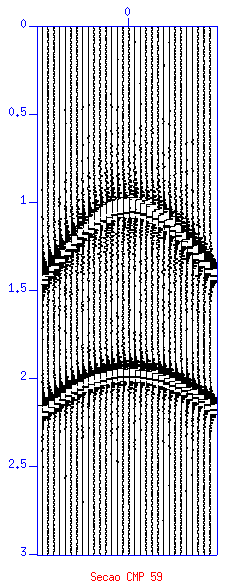
\includegraphics[width=8cm]{secao59}
	\caption{Seção CMP 59.} \label{fig:secao53}
\end{figure} 

\begin{figure}[ht!]
	\centering
	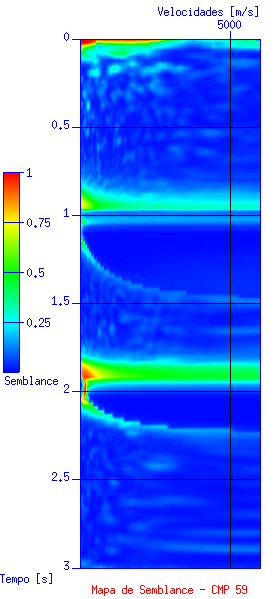
\includegraphics[width=8cm]{semblance59}
	\caption{Mapa de Semblance - CMP 59.} \label{fig:semblance59}
\end{figure}

\begin{figure}[ht!]
	\centering
	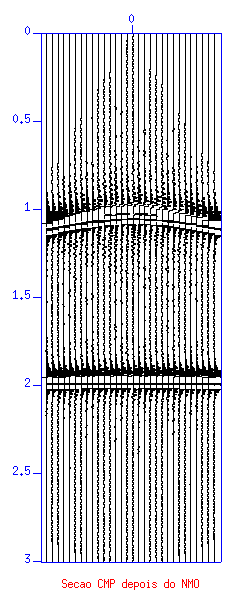
\includegraphics[width=8cm]{secao59nmo}
	\caption{Seção CMP 59 após correção NMO.} \label{fig:secao59nmo}
\end{figure}

\begin{figure}[ht!]
	\centering
	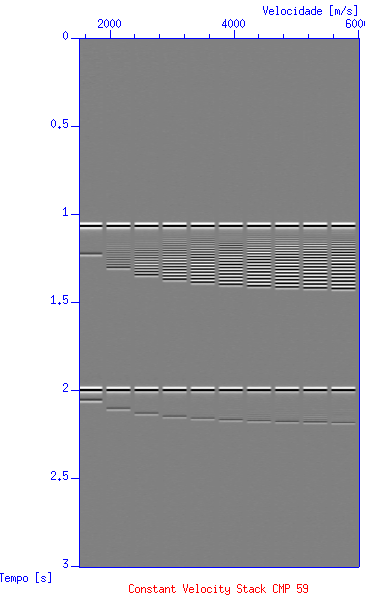
\includegraphics[width=10cm]{stackruido}
	\caption{Velocidade constante empilhada - CMP 59.} \label{fig:stackruido}
\end{figure}

\section{Aplicando ruído nos dados}

Para os próximos passos, foi aplicado ruído de Gauss nos dados de CMPs e, como comparativo, foram geradas as imagens da seção CMP 53 com o intuito de comparar as diferenças (Fig. \ref{fig:secaoruido}, Fig. \ref{fig:semblanceruido}, Fig. \ref{fig:secaohruido} e Fig. \ref{fig:velocityruido}).

\begin{figure}[ht!]
	\centering
	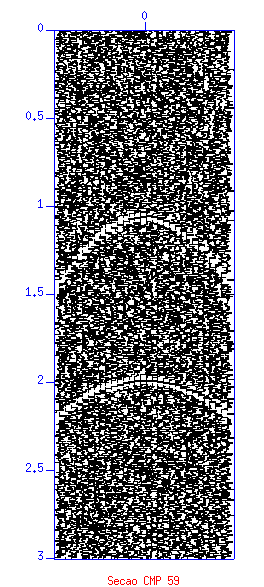
\includegraphics[width=8cm]{secaoruido}
	\caption{Seção CMP 59 com ruído.} \label{fig:secaoruido}
\end{figure} 

\begin{figure}[ht!]
	\centering
	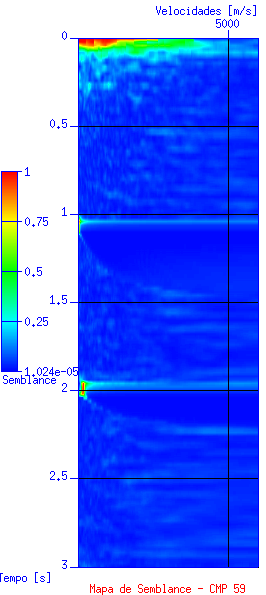
\includegraphics[width=8cm]{semblanceruido}
	\caption{Mapa de Semblance com ruído - CMP 59.} \label{fig:semblanceruido}
\end{figure}

\begin{figure}[ht!]
	\centering
	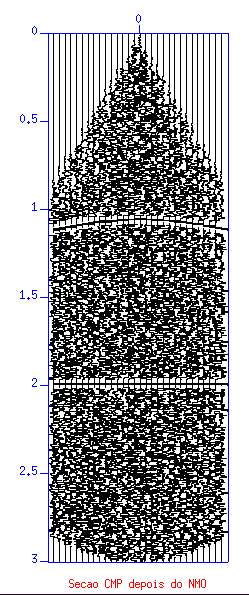
\includegraphics[width=8cm]{secaohruido}
	\caption{Seção CMP 59  com ruído após correção NMO.} \label{fig:secaohruido}
\end{figure}

\begin{figure}[ht!]
	\centering
	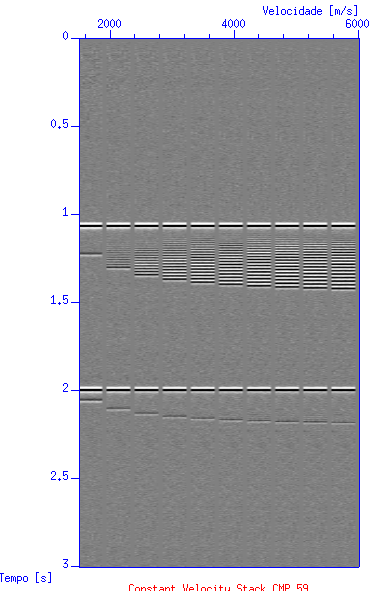
\includegraphics[width=10cm]{velocityruido}
	\caption{Velocidade constante empilhada com ruído- CMP 59.} \label{fig:velocityruido}
\end{figure}

Para comparar melhor esses testes, é possível analisar as Figuras \ref{fig:semblance59} e \ref{fig:semblanceruido}. Nota-se que no primeiro mapa semblance está bem dividida a mudança de camadas (parte verde), enquanto que na segunda não está tão claro. Para mudar isso, é preciso aplicar correções para eliminar ao máximo o ruído. 

\section{Aplicando correções} 

Após escolher as velocidades para cada família de CMP com o intuito de corrigir a velocidade foi gerada a Figura \ref{fig:correcao}. Nesta imagem mostra uma correção das hiperboles encontradas nas seções sismicas, tendo uma horizontalização das velocidades. Após a correção, foi aplicado o empilhamento (Fig. \ref{fig:empilhamento}), reunindo todas as informações e dados corrigidos. Por fim, foi aplicada a migração, sendo um processo  que elimina difrações e mapeia os eventos em uma seção empilhada, gerando a Figura \ref{fig:mig}.


\begin{figure}[ht!]
	\centering
	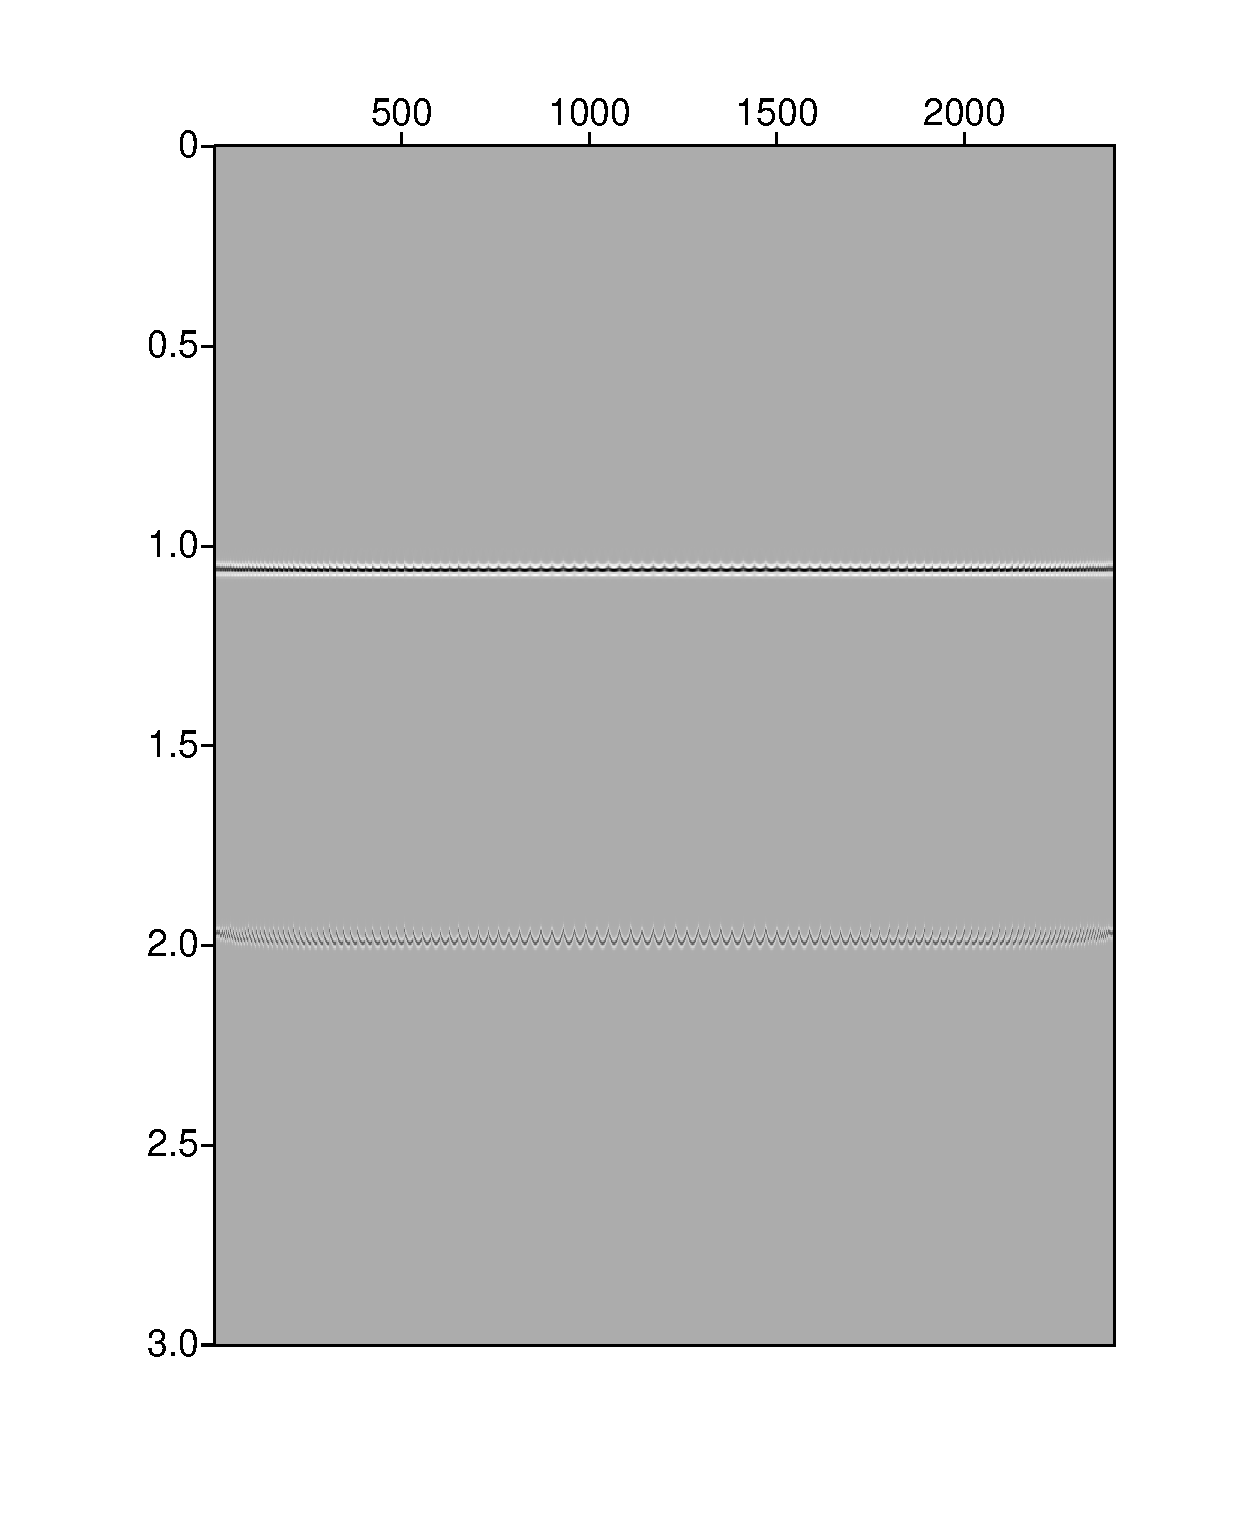
\includegraphics[width=10cm]{correção-NMO-nos-dados-CMP}
	\caption{Correção NMO.} \label{fig:correcao}
\end{figure}

\begin{figure}[ht!]
	\centering
	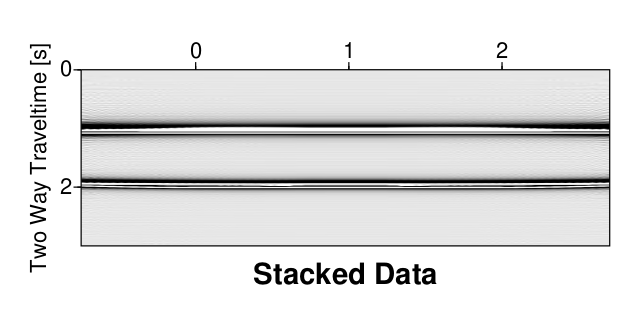
\includegraphics[width=15cm]{empilhamento}
	\caption{Empilhamento do modelo de camadas planas.} \label{fig:empilhamento}
\end{figure}

\begin{figure}[ht!]
	\centering
	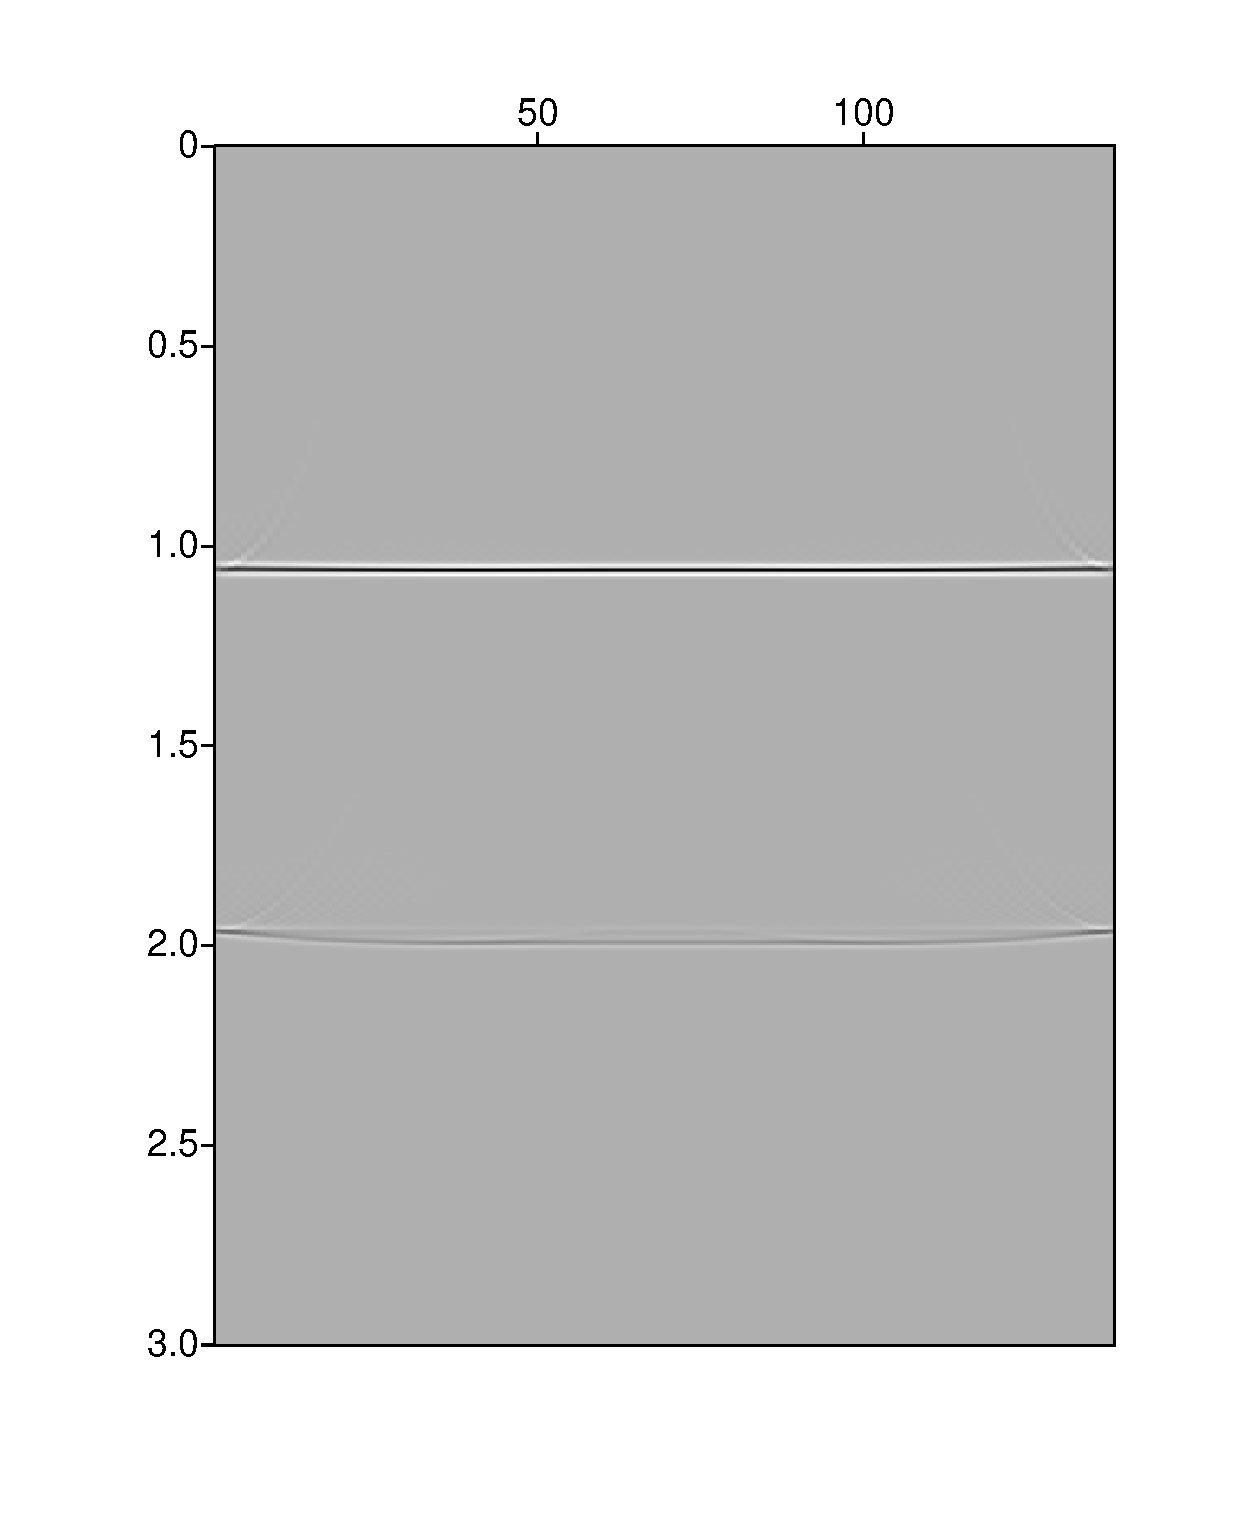
\includegraphics[width=15cm]{Migração_dos_dados}
	\caption{Migração temporal dos dados.} \label{fig:mig}
\end{figure}